% !TeX program = pdflatex
% !TeX root = FCLoopIntegralToGraph.tex

\documentclass[../FeynCalcManual.tex]{subfiles}
\begin{document}
\begin{Shaded}
\begin{Highlighting}[]
 
\end{Highlighting}
\end{Shaded}

\hypertarget{fcloopintegraltograph}{
\section{FCLoopIntegralToGraph}\label{fcloopintegraltograph}\index{FCLoopIntegralToGraph}}

\texttt{FCLoopIntegralToGraph[\allowbreak{}int,\ \allowbreak{}\{\allowbreak{}q1,\ \allowbreak{}q2,\ \allowbreak{}...\}]}
constructs a graph representation of the loop integral \texttt{int} that
depends on the loop momenta
\texttt{q1,\ \allowbreak{}q2,\ \allowbreak{}...}. The function returns a
list of the form
\texttt{\{\allowbreak{}edges,\ \allowbreak{}labels,\ \allowbreak{}props,\ \allowbreak{}pref\}},
where \texttt{edges} is a list of edge rules representing the loop
integral \texttt{int}, \texttt{labels} is a list of lists containing the
line momentum, multiplicity and the mass term of each propagator,
\texttt{props} is a list with the original propagators and \texttt{pref}
is the piece of the integral that was ignored when constructing the
graph representation (e.g.~scalar products or vectors in the numerator)
.

Use \texttt{FCLoopGraphPlot} to visualize the output of
\texttt{FCLoopIntegralToGraph}.

A quick and simple way to plot the graph is to evaluate
\texttt{GraphPlot[\allowbreak{}List @@@ Transpose[\allowbreak{}output[\allowbreak{}[\allowbreak{}1 ;; 2]]]]}
or
\texttt{GraphPlot[\allowbreak{}Labeled @@@ Transpose[\allowbreak{}output[\allowbreak{}[\allowbreak{}1 ;; 2]]]]}.
The visual quality will not be that great, though. To obtain a nicer
plot one might use \texttt{GraphPlot} with a custom
\texttt{EdgeTaggedGraph} or export the output to a file and visualize it
with an external tool such as dot/neato from
\href{https://graphviz.org/}{graphviz}.

It is also possible to invoke the function as
\texttt{FCLoopIntegralToGraph[\allowbreak{}GLI[\allowbreak{}...],\ \allowbreak{}FCTopology[\allowbreak{}...]]}
or
\texttt{FCLoopIntegralToGraph[\allowbreak{}FCTopology[\allowbreak{}...]]}.

\subsection{See also}

\hyperlink{toc}{Overview}, \hyperlink{fcloopgraphplot}{FCLoopGraphPlot}.

\subsection{Examples}

\begin{Shaded}
\begin{Highlighting}[]
\FunctionTok{out} \ExtensionTok{=}\NormalTok{ FCLoopIntegralToGraph}\OperatorTok{[}\NormalTok{FAD}\OperatorTok{[\{}\FunctionTok{q} \SpecialCharTok{{-}}\NormalTok{ k1}\OperatorTok{\},}\NormalTok{ k1}\OperatorTok{,} \FunctionTok{q} \SpecialCharTok{{-}}\NormalTok{ k2}\OperatorTok{,}\NormalTok{ k2}\OperatorTok{,} \OperatorTok{\{}\NormalTok{k2 }\SpecialCharTok{{-}}\NormalTok{ k3}\OperatorTok{,}\NormalTok{ mb}\OperatorTok{\},} \OperatorTok{\{}\NormalTok{k1 }\SpecialCharTok{{-}}\NormalTok{ k3}\OperatorTok{,}\NormalTok{ mb}\OperatorTok{\}],} \OperatorTok{\{}\NormalTok{k1}\OperatorTok{,}\NormalTok{ k2}\OperatorTok{,}\NormalTok{ k3}\OperatorTok{\}]}
\end{Highlighting}
\end{Shaded}

\begin{dmath*}\breakingcomma
\left\{\{-3\to 2,-1\to 1,1\to 3,1\to 4,2\to 3,2\to 4,3\to 4,3\to 4\},\left\{-q,q,\{\text{k2},1,0\},\{q-\text{k2},1,0\},\{\text{k1},1,0\},\{q-\text{k1},1,0\},\left\{\text{k2}-\text{k3},1,-\text{mb}^2\right\},\left\{\text{k1}-\text{k3},1,-\text{mb}^2\right\}\right\},\left\{0,0,\frac{1}{(\text{k2}^2+i \eta )},\frac{1}{(\text{k1}^2+i \eta )},\frac{1}{((q-\text{k2})^2+i \eta )},\frac{1}{((q-\text{k1})^2+i \eta )},\frac{1}{((\text{k2}-\text{k3})^2-\text{mb}^2+i \eta )},\frac{1}{((\text{k1}-\text{k3})^2-\text{mb}^2+i \eta )}\right\},1\right\}
\end{dmath*}

\begin{Shaded}
\begin{Highlighting}[]
\NormalTok{FCLoopGraphPlot}\OperatorTok{[}\FunctionTok{out}\OperatorTok{]}
\end{Highlighting}
\end{Shaded}

\FloatBarrier
\begin{figure}[!ht]
\centering
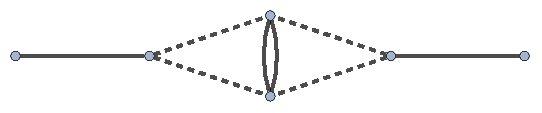
\includegraphics[width=0.6\linewidth]{img/0bfm86ewusrdi.pdf}
\end{figure}
\FloatBarrier

\begin{Shaded}
\begin{Highlighting}[]
\FunctionTok{Labeled}\NormalTok{ @@@ }\FunctionTok{Transpose}\OperatorTok{[}\FunctionTok{out}\OperatorTok{[[}\DecValTok{1}\NormalTok{ ;; }\DecValTok{2}\OperatorTok{]]]}
\end{Highlighting}
\end{Shaded}

\FloatBarrier
\begin{figure}[!ht]
\centering
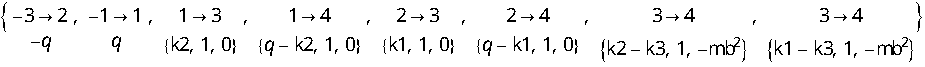
\includegraphics[width=0.6\linewidth]{img/01p715ugi4jrv.pdf}
\end{figure}
\FloatBarrier

\begin{Shaded}
\begin{Highlighting}[]
\FunctionTok{GraphPlot}\OperatorTok{[}\FunctionTok{List}\NormalTok{ @@@ }\FunctionTok{Transpose}\OperatorTok{[}\FunctionTok{out}\OperatorTok{[[}\DecValTok{1}\NormalTok{ ;; }\DecValTok{2}\OperatorTok{]]]]}
\end{Highlighting}
\end{Shaded}

\FloatBarrier
\begin{figure}[!ht]
\centering
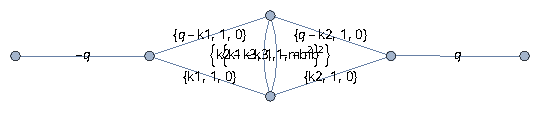
\includegraphics[width=0.6\linewidth]{img/0blv15cgm9d0u.pdf}
\end{figure}
\FloatBarrier

\begin{Shaded}
\begin{Highlighting}[]
\NormalTok{FCLoopIntegralToGraph}\OperatorTok{[}\NormalTok{FAD}\OperatorTok{[\{}\FunctionTok{q} \SpecialCharTok{{-}}\NormalTok{ k1}\OperatorTok{\},}\NormalTok{ k1}\OperatorTok{,} \FunctionTok{q} \SpecialCharTok{{-}}\NormalTok{ k2}\OperatorTok{,}\NormalTok{ k2}\OperatorTok{,} \OperatorTok{\{}\NormalTok{k2 }\SpecialCharTok{{-}}\NormalTok{ k3}\OperatorTok{,}\NormalTok{ mb}\OperatorTok{\},} \OperatorTok{\{}\NormalTok{k1 }\SpecialCharTok{{-}}\NormalTok{ k3}\OperatorTok{,}\NormalTok{ mb}\OperatorTok{\}],} \OperatorTok{\{}\NormalTok{k1}\OperatorTok{,}\NormalTok{ k2}\OperatorTok{,}\NormalTok{k3}\OperatorTok{\}]}
\end{Highlighting}
\end{Shaded}

\begin{dmath*}\breakingcomma
\left\{\{-3\to 2,-1\to 1,1\to 3,1\to 4,2\to 3,2\to 4,3\to 4,3\to 4\},\left\{-q,q,\{\text{k2},1,0\},\{q-\text{k2},1,0\},\{\text{k1},1,0\},\{q-\text{k1},1,0\},\left\{\text{k2}-\text{k3},1,-\text{mb}^2\right\},\left\{\text{k1}-\text{k3},1,-\text{mb}^2\right\}\right\},\left\{0,0,\frac{1}{(\text{k2}^2+i \eta )},\frac{1}{(\text{k1}^2+i \eta )},\frac{1}{((q-\text{k2})^2+i \eta )},\frac{1}{((q-\text{k1})^2+i \eta )},\frac{1}{((\text{k2}-\text{k3})^2-\text{mb}^2+i \eta )},\frac{1}{((\text{k1}-\text{k3})^2-\text{mb}^2+i \eta )}\right\},1\right\}
\end{dmath*}

\begin{Shaded}
\begin{Highlighting}[]
\NormalTok{FAD}\OperatorTok{[}\FunctionTok{q} \SpecialCharTok{{-}}\NormalTok{ k1}\OperatorTok{,}\NormalTok{ k1}\OperatorTok{,} \FunctionTok{q} \SpecialCharTok{{-}}\NormalTok{ k2}\OperatorTok{,}\NormalTok{ k2}\OperatorTok{,} \OperatorTok{\{}\NormalTok{k2 }\SpecialCharTok{{-}}\NormalTok{ k3}\OperatorTok{,}\NormalTok{ mb}\OperatorTok{\},} \OperatorTok{\{}\NormalTok{k1 }\SpecialCharTok{{-}}\NormalTok{ k3}\OperatorTok{,}\NormalTok{ mb}\OperatorTok{\}]}
\end{Highlighting}
\end{Shaded}

\begin{dmath*}\breakingcomma
\frac{1}{(q-\text{k1})^2.\text{k1}^2.(q-\text{k2})^2.\text{k2}^2.\left((\text{k2}-\text{k3})^2-\text{mb}^2\right).\left((\text{k1}-\text{k3})^2-\text{mb}^2\right)}
\end{dmath*}

If the input is given as a list of propagators, their ordering will be
preserved when constructing the graph

\begin{Shaded}
\begin{Highlighting}[]
\NormalTok{FCLoopIntegralToGraph}\OperatorTok{[}\NormalTok{FCTopology}\OperatorTok{[}\NormalTok{topo1}\OperatorTok{,} \OperatorTok{\{}\NormalTok{FAD}\OperatorTok{[}\FunctionTok{q} \SpecialCharTok{{-}}\NormalTok{ k1}\OperatorTok{],}\NormalTok{ FAD}\OperatorTok{[}\NormalTok{k1}\OperatorTok{],}\NormalTok{ FAD}\OperatorTok{[}\FunctionTok{q} \SpecialCharTok{{-}}\NormalTok{ k2}\OperatorTok{],}\NormalTok{ FAD}\OperatorTok{[}\NormalTok{k2}\OperatorTok{],} 
\NormalTok{    FAD}\OperatorTok{[\{}\NormalTok{k2 }\SpecialCharTok{{-}}\NormalTok{ k3}\OperatorTok{,}\NormalTok{ mb}\OperatorTok{\}],}\NormalTok{ FAD}\OperatorTok{[\{}\NormalTok{k1 }\SpecialCharTok{{-}}\NormalTok{ k3}\OperatorTok{,}\NormalTok{ mb}\OperatorTok{\}]\},} \OperatorTok{\{}\NormalTok{k1}\OperatorTok{,}\NormalTok{ k2}\OperatorTok{,}\NormalTok{ k3}\OperatorTok{\},} \OperatorTok{\{}\FunctionTok{q}\OperatorTok{\},} \OperatorTok{\{\},} \OperatorTok{\{\}]]}
\end{Highlighting}
\end{Shaded}

\begin{dmath*}\breakingcomma
\left\{\{-3\to 2,-1\to 1,1\to 3,1\to 4,2\to 3,2\to 4,3\to 4,3\to 4\},\left\{-q,q,\{q-\text{k1},1,0\},\{\text{k1},1,0\},\{q-\text{k2},1,0\},\{\text{k2},1,0\},\left\{\text{k2}-\text{k3},1,-\text{mb}^2\right\},\left\{\text{k1}-\text{k3},1,-\text{mb}^2\right\}\right\},\left\{0,0,\frac{1}{((q-\text{k1})^2+i \eta )},\frac{1}{(\text{k1}^2+i \eta )},\frac{1}{((q-\text{k2})^2+i \eta )},\frac{1}{(\text{k2}^2+i \eta )},\frac{1}{((\text{k2}-\text{k3})^2-\text{mb}^2+i \eta )},\frac{1}{((\text{k1}-\text{k3})^2-\text{mb}^2+i \eta )}\right\},1\right\}
\end{dmath*}

\begin{Shaded}
\begin{Highlighting}[]
\NormalTok{FCLoopIntegralToGraph}\OperatorTok{[}\NormalTok{GLI}\OperatorTok{[}\NormalTok{topo1}\OperatorTok{,} \OperatorTok{\{}\DecValTok{1}\OperatorTok{,} \DecValTok{1}\OperatorTok{,} \DecValTok{1}\OperatorTok{,} \DecValTok{1}\OperatorTok{,} \DecValTok{1}\OperatorTok{,} \DecValTok{1}\OperatorTok{\}],} 
\NormalTok{  FCTopology}\OperatorTok{[}\NormalTok{topo1}\OperatorTok{,} \OperatorTok{\{}\NormalTok{FAD}\OperatorTok{[}\FunctionTok{q} \SpecialCharTok{{-}}\NormalTok{ k1}\OperatorTok{],}\NormalTok{ FAD}\OperatorTok{[}\NormalTok{k1}\OperatorTok{],}\NormalTok{ FAD}\OperatorTok{[}\FunctionTok{q} \SpecialCharTok{{-}}\NormalTok{ k2}\OperatorTok{],}\NormalTok{ FAD}\OperatorTok{[}\NormalTok{k2}\OperatorTok{],} 
\NormalTok{    FAD}\OperatorTok{[\{}\NormalTok{k2 }\SpecialCharTok{{-}}\NormalTok{ k3}\OperatorTok{,}\NormalTok{ mb}\OperatorTok{\}],}\NormalTok{ FAD}\OperatorTok{[\{}\NormalTok{k1 }\SpecialCharTok{{-}}\NormalTok{ k3}\OperatorTok{,}\NormalTok{ mb}\OperatorTok{\}]\},} \OperatorTok{\{}\NormalTok{k1}\OperatorTok{,}\NormalTok{ k2}\OperatorTok{,}\NormalTok{ k3}\OperatorTok{\},} \OperatorTok{\{}\FunctionTok{q}\OperatorTok{\},} \OperatorTok{\{\},} \OperatorTok{\{\}]]}
\end{Highlighting}
\end{Shaded}

\begin{dmath*}\breakingcomma
\left\{\{-3\to 2,-1\to 1,1\to 3,1\to 4,2\to 3,2\to 4,3\to 4,3\to 4\},\left\{-q,q,\{\text{k2},1,0\},\{q-\text{k2},1,0\},\{\text{k1},1,0\},\{q-\text{k1},1,0\},\left\{\text{k2}-\text{k3},1,-\text{mb}^2\right\},\left\{\text{k1}-\text{k3},1,-\text{mb}^2\right\}\right\},\left\{0,0,\frac{1}{(\text{k2}^2+i \eta )},\frac{1}{(\text{k1}^2+i \eta )},\frac{1}{((q-\text{k2})^2+i \eta )},\frac{1}{((q-\text{k1})^2+i \eta )},\frac{1}{((\text{k2}-\text{k3})^2-\text{mb}^2+i \eta )},\frac{1}{((\text{k1}-\text{k3})^2-\text{mb}^2+i \eta )}\right\},1\right\}
\end{dmath*}

If the second argument contains multiple topologies, the function will
automatically select the relevant ones.

\begin{Shaded}
\begin{Highlighting}[]
\NormalTok{FCLoopIntegralToGraph}\OperatorTok{[}\NormalTok{GLI}\OperatorTok{[}\NormalTok{topo1}\OperatorTok{,} \OperatorTok{\{}\DecValTok{1}\OperatorTok{,} \DecValTok{1}\OperatorTok{,} \DecValTok{1}\OperatorTok{,} \DecValTok{0}\OperatorTok{,} \DecValTok{0}\OperatorTok{,} \DecValTok{0}\OperatorTok{\}],} 
  \OperatorTok{\{}\NormalTok{FCTopology}\OperatorTok{[}\NormalTok{topo1}\OperatorTok{,} \OperatorTok{\{}\NormalTok{FAD}\OperatorTok{[}\FunctionTok{q} \SpecialCharTok{{-}}\NormalTok{ k1}\OperatorTok{],}\NormalTok{ FAD}\OperatorTok{[}\NormalTok{k1}\OperatorTok{],}\NormalTok{ FAD}\OperatorTok{[}\FunctionTok{q} \SpecialCharTok{{-}}\NormalTok{ k2}\OperatorTok{],}\NormalTok{ FAD}\OperatorTok{[}\NormalTok{k2}\OperatorTok{],} 
\NormalTok{     FAD}\OperatorTok{[\{}\NormalTok{k2 }\SpecialCharTok{{-}}\NormalTok{ k3}\OperatorTok{,}\NormalTok{ mb}\OperatorTok{\}],}\NormalTok{ FAD}\OperatorTok{[\{}\NormalTok{k1 }\SpecialCharTok{{-}}\NormalTok{ k3}\OperatorTok{,}\NormalTok{ mb}\OperatorTok{\}]\},} \OperatorTok{\{}\NormalTok{k1}\OperatorTok{,}\NormalTok{ k2}\OperatorTok{,}\NormalTok{ k3}\OperatorTok{\},} \OperatorTok{\{}\FunctionTok{q}\OperatorTok{\},} \OperatorTok{\{\},} \OperatorTok{\{\}],} 
\NormalTok{   FCTopology}\OperatorTok{[}\NormalTok{topo2}\OperatorTok{,} \OperatorTok{\{}\NormalTok{FAD}\OperatorTok{[}\FunctionTok{q} \SpecialCharTok{{-}}\NormalTok{ k1}\OperatorTok{],}\NormalTok{ FAD}\OperatorTok{[}\NormalTok{k1}\OperatorTok{],}\NormalTok{ FAD}\OperatorTok{[}\FunctionTok{q} \SpecialCharTok{{-}}\NormalTok{ k2}\OperatorTok{],}\NormalTok{ FAD}\OperatorTok{[}\NormalTok{k2}\OperatorTok{],} 
\NormalTok{     FAD}\OperatorTok{[\{}\NormalTok{k2 }\SpecialCharTok{{-}}\NormalTok{ k3}\OperatorTok{,}\NormalTok{ mg}\OperatorTok{\}],}\NormalTok{ FAD}\OperatorTok{[\{}\NormalTok{k1 }\SpecialCharTok{{-}}\NormalTok{ k3}\OperatorTok{,}\NormalTok{ mg}\OperatorTok{\}]\},} \OperatorTok{\{}\NormalTok{k1}\OperatorTok{,}\NormalTok{ k2}\OperatorTok{,}\NormalTok{ k3}\OperatorTok{\},} \OperatorTok{\{}\FunctionTok{q}\OperatorTok{\},} \OperatorTok{\{\},} \OperatorTok{\{\}]} 
  \OperatorTok{\}]}
\end{Highlighting}
\end{Shaded}

\begin{dmath*}\breakingcomma
\left\{\{-3\to 2,-1\to 1,1\to 2,1\to 2,2\to 2\},\{-q,q,\{\text{k1},1,0\},\{q-\text{k1},1,0\},\{q-\text{k2},1,0\}\},\left\{0,0,\frac{1}{(\text{k1}^2+i \eta )},\frac{1}{((q-\text{k2})^2+i \eta )},\frac{1}{((q-\text{k1})^2+i \eta )}\right\},1\right\}
\end{dmath*}
\end{document}
